\documentclass{beamer}

\usetheme{Madrid}
\usepackage{amsmath, amssymb}
\usepackage{algpseudocode}
\usepackage{graphicx}

\newtheorem{assumption}{Assumption}

\title{Proximal Drift-Plus-Penalty}
\subtitle{Numerical Validation}
\author{}
\date{\today}

\begin{document}

\begin{frame}
  \titlepage
\end{frame}

% ------------------------------------------------------------------
\begin{frame}{Overview}
  \small
  \textbf{Primal problem:}
  \[
    \min_{x \in X} f(x) \quad \text{s.t.} \quad g(x) \le 0,\ h(x) \le 0
  \]

  \textbf{Penalized objective:}
  \[
    P(x) = f(x) + \beta\,[g(x)]_+
  \]

  \textbf{Algorithm (per step $t$, $q_t := Q_t/V$):}
  \begin{align*}
    x_{t+1} &= \operatorname*{arg\,min}_{x \in X} P(x) + q_t\big(h(x)+\gamma\|x-x_t\|^2\big) + \tfrac{1}{2\eta}\|x-x_t\|^2 \\
    Q_{t+1} &= \max(Q_t + h(x_{t+1}),\,0)
  \end{align*}

  \vspace{0.5em}
  \begin{block}{Observation}
    \small The queue stays bounded, the time-average of $h$ vanishes at rate $O(V/t)$, the average movement $\|x_{t+1}-x_t\|^2$ at rate $O(1/t+1/V)$, and $[g(x)]_+$ sits at floating-point noise -- matching every predicted rate.
  \end{block}
\end{frame}

% ------------------------------------------------------------------
\begin{frame}{Domain}
  \[
    X = \{\, x \in \mathbb{R}^d : \|x\| \le R_X \,\} \qquad D := \operatorname{diam}(X) = 2R_X
  \]

  \[
    f(x) = \tfrac{1}{2} x^\top \mathrm{diag}(w^f_{\mathrm{quad}})\, x \;-\; c_f^\top x \;+\; \sum_{j=1}^{4} \alpha^f_j \cos\big(w^f_j \cdot x + b^f_j\big)
  \]

  \[
    h(x) = \tfrac{1}{2} x^\top \mathrm{diag}(w^h_{\mathrm{quad}})\, x \;+\; \sum_{j=1}^{2} \alpha^h_j \cos\big(w^h_j \cdot x + b^h_j\big) \;+\; \text{offset}_h
  \]

  \[
    g(x) = \|x\|^2 - r_g^2
  \]

  \begin{itemize}
    \item $f, h$: weakly convex (a quadratic plus a bounded cosine perturbation)
    \item $g$: instantaneous ball-violation term, no randomness
  \end{itemize}
\end{frame}

% ------------------------------------------------------------------
\begin{frame}{Synthetic Instance: Exact Coefficients}
  \small
  $d=10$, \ $R_X=1$, \ $r_g=0.75$ ($r_g^2=0.5625$), \ $\xi=0.4$, \ $D=2$, \ seed $=0$

  \vspace{0.3em}
  $w^f_{\mathrm{quad},i}=0.2\ \forall i$, \ $\alpha^f=(0.015,0.015,0.015,0.015)$, \ $b_f=(4.0021,1.6951,0.2574,0.1038)$, \ offset$_f=0$

  \vspace{0.3em}
  $w^h_{\mathrm{quad},i}=2.0\ \forall i$, \ $\alpha^h=(0.02,0.03)$, \ $b_h=(2.1119,0.9442)$, \ offset$_h=-0.4073$

  \vspace{0.5em}
  \centering
  \tiny
  \begin{tabular}{c|rrrr|r|rr}
    $i$ & $w^f_1$ & $w^f_2$ & $w^f_3$ & $w^f_4$ & $c_f$ & $w^h_1$ & $w^h_2$ \\
    \hline
    1  & -0.6009 &  0.5514 &  0.0825 &  0.0876 & -0.0809 &  0.2352 &  0.3906 \\
    2  & -0.3532 &  0.0574 &  0.1365 & -0.1040 &  0.0546 &  0.3809 &  0.3257 \\
    3  & -0.2625 & -0.4537 & -0.2511 &  0.4828 &  0.1970 & -0.6479 &  0.1563 \\
    4  & -0.1525 & -0.5625 & -0.0498 &  0.6491 &  0.1431 & -0.3621 & -0.5436 \\
    5  &  0.1985 & -0.2793 &  0.3011 &  0.5966 & -0.1063 & -0.2388 &  0.0128 \\
    6  &  0.5028 &  0.1344 &  0.5736 &  0.4355 & -0.1912 & -0.6401 &  0.1687 \\
    7  & -0.0620 & -0.6161 & -0.4836 &  0.1183 & -0.0942 &  0.9518 &  0.2477 \\
    8  &  0.6590 & -0.1277 &  0.5815 & -0.4001 &  0.0062 & -0.2714 & -0.1524 \\
    9  & -0.3208 & -0.0972 &  0.5169 & -0.0015 & -0.3512 &  0.1800 &  0.4495 \\
    10 &  0.1695 &  0.3301 &  0.3001 &  0.2174 & -0.0331 & -0.1415 & -0.3258 \\
  \end{tabular}
\end{frame}

% ------------------------------------------------------------------
\begin{frame}{Weak Convexity and Lipschitz Constants}
  \footnotesize
  \textbf{Weak convexity moduli} (upper bound on $-\lambda_{\min}(\nabla^2 \cdot)$):
  \[
    \rho_f = \sum_{j=1}^4 \alpha^f_j\|w^f_j\|^2, \qquad
    \rho_h = \sum_{j=1}^2 \alpha^h_j\|w^h_j\|^2, \qquad
    \rho_g = 0
  \]
  ($g$ is exactly convex -- a plain quadratic, no perturbation.)

  \textbf{Lipschitz bounds} on $\|\nabla(\cdot)\|$ over $\|x\| \le R_X$:
  \[
    L_f = \max(w^f_{\mathrm{quad}})R_X + \|c_f\| + \sum_{j=1}^4 \alpha^f_j\|w^f_j\|, \qquad L_g = 2R_X
  \]
  \[
    L_h = \max(w^h_{\mathrm{quad}})R_X + \sum_{j=1}^2 \alpha^h_j\|w^h_j\|
  \]

  \centering
  \begin{tabular}{c|ccc}
     & $f$ & $h$ & $g$ \\
    \hline
    $\rho$ & 0.0864 & 0.0750 & 0 \\
    $L$    & 0.7720 & 2.0600 & 2.0000 \\
  \end{tabular}

  \vspace{0.3em}
  \small
  \raggedright
  \textbf{Strong convexity of the subproblem:} $\mu = 1/\eta - \rho_f + q_t(2\gamma-\rho_h) \in [0.9136,\ 1.0283]$ over the run ($q_t \in [0,\bar q]$) -- always $>0$, so Assumption 7 holds at every step, not just initially.
\end{frame}

% ------------------------------------------------------------------
\begin{frame}{Solving the Subproblem: Proximal Gradient}
  \footnotesize
  Smooth: $S(x) = f(x) + q_t\big(h(x)+\gamma\|x-x_t\|^2\big) + \tfrac{1}{2\eta}\|x-x_t\|^2$. \quad
  Non-smooth: $\beta[g(x)]_+ + \iota_X(x)$.

  \begin{algorithmic}[1]
    \State $x_1 \gets 0,\ Q_1 \gets 0$
    \For{$t = 1, \dots, T$}
      \State $q_t \gets Q_t / V$; \quad $x \gets x_t$
      \For{$k = 1, \dots, 400$}
        \State $y \gets x - \text{step}\cdot \nabla S(x)$ \Comment{gradient step, smooth part}
        \State $x_{\text{new}} \gets \operatorname{prox}_{\text{step}\cdot(\beta[\cdot]_+ + \iota_X)}(y)$ \Comment{closed-form prox}
        \If{$\|x_{\text{new}} - x\| < 10^{-12}$}
          \State \textbf{break}
        \EndIf
        \State $x \gets x_{\text{new}}$
      \EndFor
      \State $x_{t+1} \gets x,\quad Q_{t+1} \gets \max(Q_t + h(x_{t+1}),\, 0)$
    \EndFor
  \end{algorithmic}

  \texttt{step}$=1/L$, $L=\text{smooth}_f+q_t\text{smooth}_h+2\gamma q_t+1/\eta=0.2864+2.155\,q_t$: \ $L{=}1.2864,\text{step}{=}0.777$ at $t{=}1$; \ $L{\approx}1.925,\text{step}{\approx}0.519$ at steady state ($q_t{\to}0.2964$, far below the worst-case ceiling $\bar q{\approx}22.94$, which would give $L{=}50.72$).

  Both $g$, $X$ are radial, so their joint prox is closed-form in $\|x\|$.
\end{frame}

% ------------------------------------------------------------------
\begin{frame}{Experimental Setup}
  \textbf{Synthetic instance:} $d=10$, $R_X=1$, $r_g=0.75$, $\xi=0.4$, seed $=0$

  \vspace{0.5em}
  \textbf{Default operating point:} $\beta=45$, $\gamma=0.04$, $\eta=1.0$, $V=20$, $T=600$

  \vspace{0.5em}
  \textbf{Solver:} entirely hand-rolled in \texttt{numpy} -- no \texttt{scipy.optimize}, \texttt{CVXPY}, or autodiff.
  \begin{itemize}
    \item Gradients written by hand (\texttt{WeaklyConvexTerm.grad}, \texttt{Problem.grad\_f/grad\_h/grad\_g})
    \item Prox step is the closed-form \texttt{\_prox\_hinge\_ball}, also derived and written by hand
    \item Up to 400 inner iterations per outer step, tolerance $10^{-12}$
  \end{itemize}
\end{frame}

% ------------------------------------------------------------------
\begin{frame}{Sweep Grids}
  \begin{itemize}
    \item $V \in \{2, 5, 10, 20, 40, 80\}$ \quad ($\beta,\gamma,\eta$ at default, $T=600$) -- Lemma 2 / Theorems 1--3
    \item $\beta \in \{25, 35, 50, 70\}$ \quad ($\gamma,\eta,V,T$ at default) -- ablation
    \item $\gamma \in \{0.04, 0.055, 0.07, 0.09\}$ \quad ($\beta,\eta,V,T$ at default) -- ablation
    \item $\eta \in \{0.3, 0.6, 1.0, 1.5\}$ \quad ($\beta,\gamma,V,T$ at default) -- ablation
    \item $\varepsilon \in \{0.3, 0.2, 0.15, 0.1, 0.08, 0.05, 0.03, 0.02\}$, $V=\lceil\varepsilon^{-2}\rceil$, $T=\lceil\varepsilon^{-3}\rceil$ -- Corollary 1
  \end{itemize}
\end{frame}

% ------------------------------------------------------------------
\begin{frame}{Ablation -- $\beta$}
  \begin{columns}[T]
    \begin{column}{0.48\textwidth}
      \small
      $\beta \in \{25, 35, 50, 70\}$, others fixed at default.

      \vspace{0.5em}
      All four final metrics (avg $h(x)$, avg movement$^2$, avg residual$^2$, avg $[g(x)]_+$) are flat.

      \vspace{0.5em}
      \textbf{Why:} the iterates never leave $\{g\le0\}$ (beyond roundoff), so the penalty $\beta[g]_+$ is never active and the trajectory does not depend on $\beta$. The \emph{bounds} do: $\beta$ enters Theorems 1(b) and 2 through $C_S$ (via $P_{\max}(\beta)$), and Theorem 3 through $\kappa_g = 2\beta r_g$. Lemma 2 and Theorem 1(a) do not depend on $\beta$.

      \vspace{0.5em}
      \textbf{Chosen:} $\beta=45$.
    \end{column}
    \begin{column}{0.52\textwidth}
      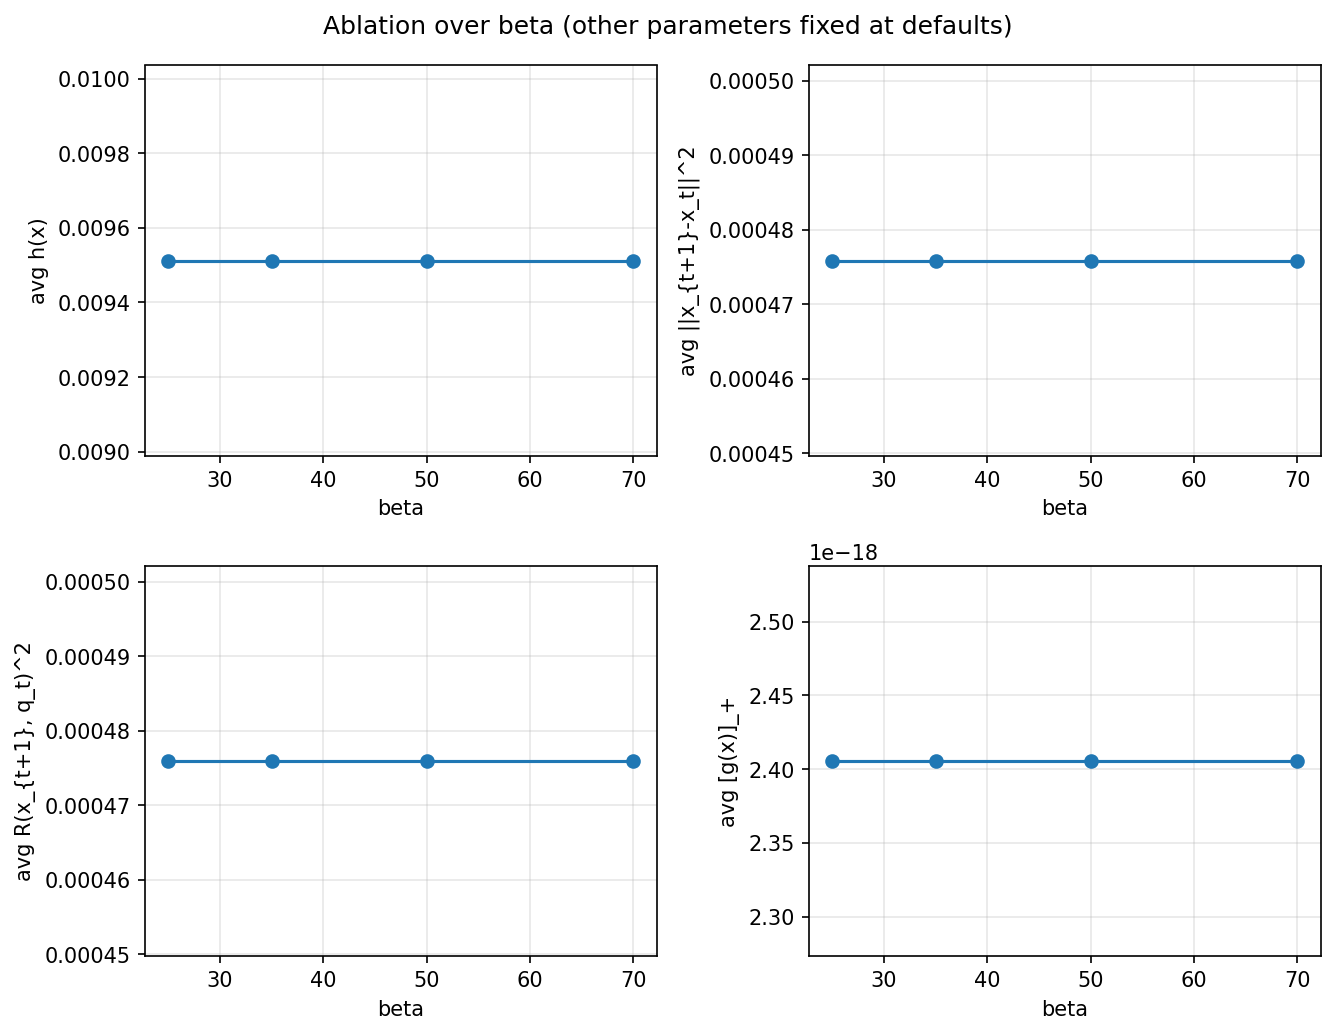
\includegraphics[width=\linewidth]{../figures/static/ablation_beta.png}
    \end{column}
  \end{columns}
\end{frame}

% ------------------------------------------------------------------
\begin{frame}{Ablation -- $\gamma$}
  \begin{columns}[T]
    \begin{column}{0.48\textwidth}
      \small
      $\gamma \in \{0.04, 0.055, 0.07, 0.09\}$, window $(\rho_h/2,\ \xi/D^2) = (0.0375,\ 0.1)$.

      \vspace{0.5em}
      All four final metrics are essentially flat: avg $h(x)$ and avg movement$^2$ agree to 5 significant figures, avg residual$^2$ rises by only $\approx0.02\%$ ($4.7592\to4.7602\times10^{-4}$), and $[g(x)]_+$ stays at roundoff -- $\gamma$'s effect is negligible at this operating point.

      \vspace{0.5em}
      \textbf{Chosen:} $\gamma=0.04$ -- near the low end of the window, leaving most of the Slater margin unconsumed.
    \end{column}
    \begin{column}{0.52\textwidth}
      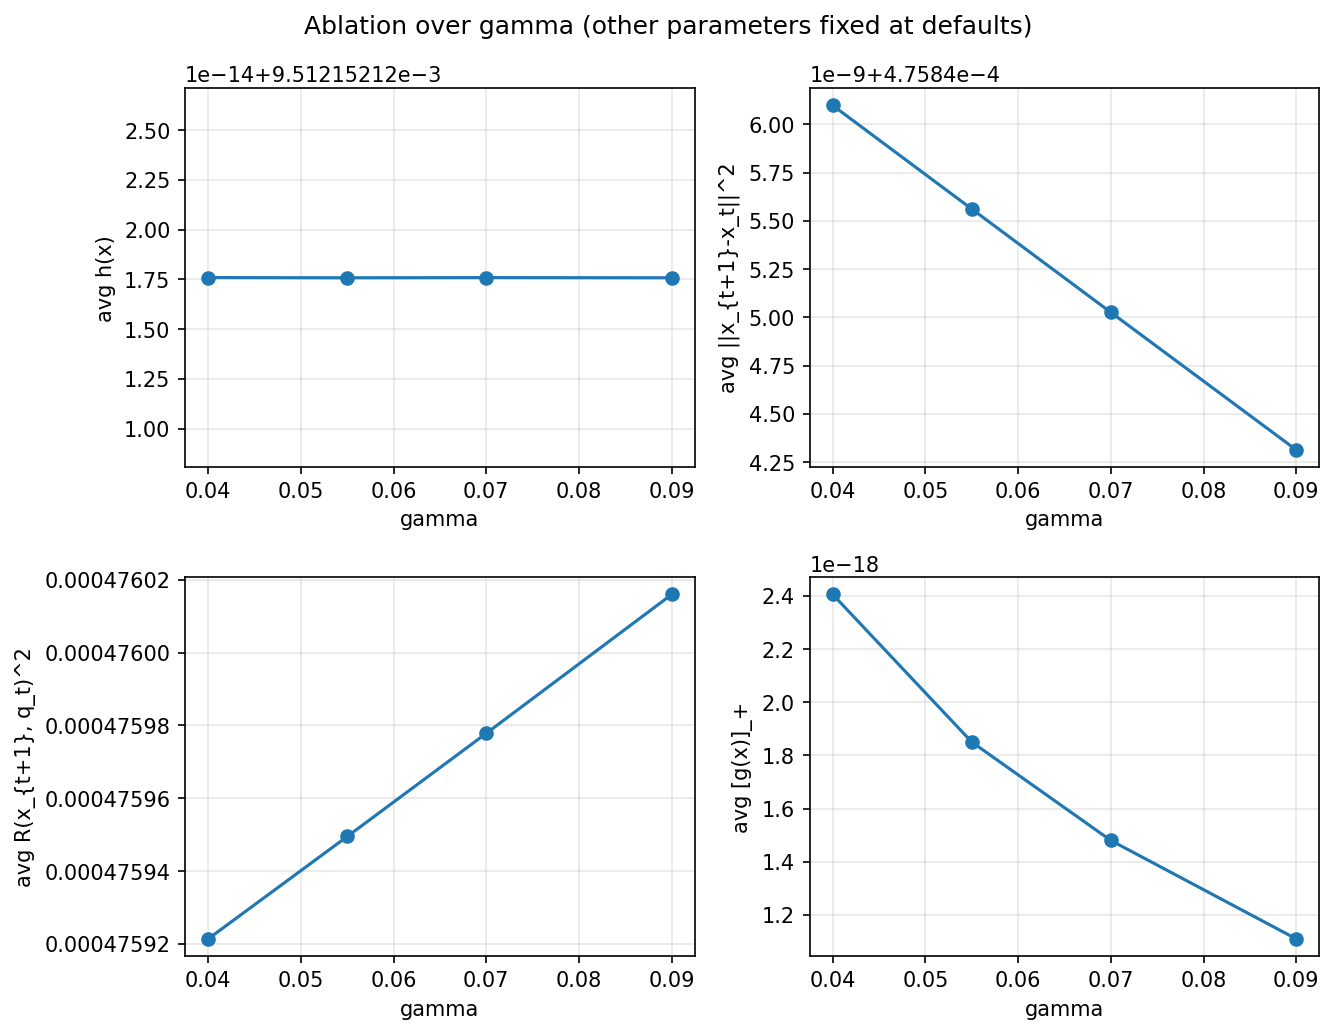
\includegraphics[width=\linewidth]{../figures/static/ablation_gamma.png}
    \end{column}
  \end{columns}
\end{frame}

% ------------------------------------------------------------------
\begin{frame}{Ablation -- $\eta$}
  \begin{columns}[T]
    \begin{column}{0.48\textwidth}
      \small
      $\eta \in \{0.3, 0.6, 1.0, 1.5\}$, window $(0,\ 1/\rho_f) = (0,\ 11.57)$.

      \vspace{0.5em}
      Larger $\eta$ widens the effective step: avg $h(x)$ and movement both increase, but avg residual$^2$ \emph{decreases}, since $R = A_t\cdot\text{movement}$ and $A_t = 1/\eta + 2\gamma q_t$ shrinks faster than movement grows. $[g(x)]_+$ stays at floating-point scale throughout.

      \vspace{0.5em}
      \textbf{Chosen:} $\eta=1.0$ -- keeps $D^2/(2\eta)$, and hence $\bar q$, small.
    \end{column}
    \begin{column}{0.52\textwidth}
      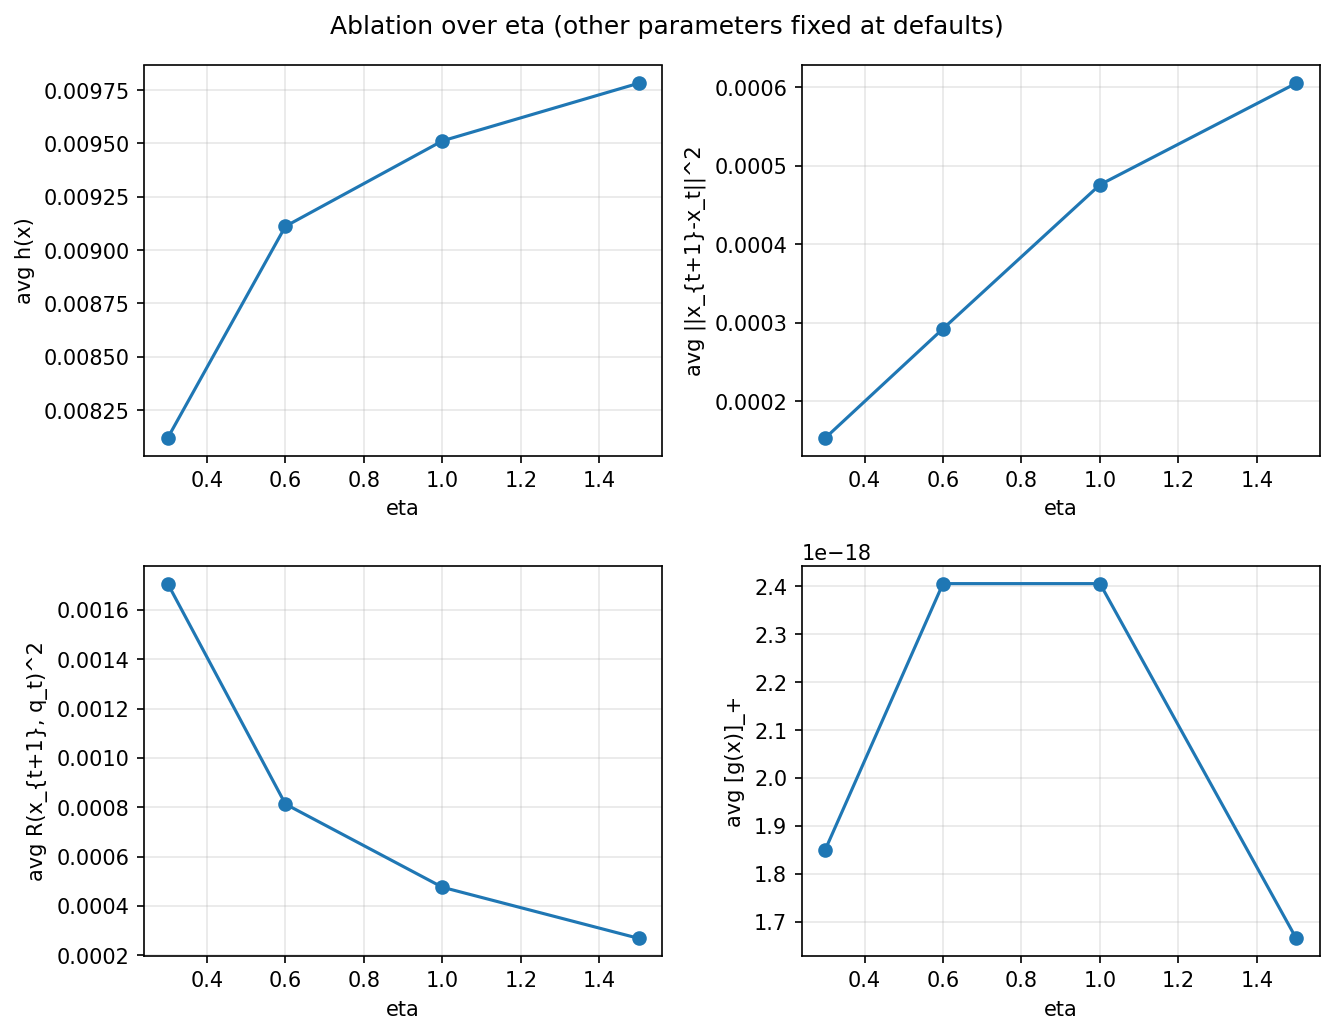
\includegraphics[width=\linewidth]{../figures/static/ablation_eta.png}
    \end{column}
  \end{columns}
\end{frame}

% ------------------------------------------------------------------
\begin{frame}{Lemma 2: Queue Boundedness}
  \begin{columns}[T]
    \begin{column}{0.48\textwidth}
      \footnotesize
      \[
        Q_t \;\le\; \frac{2V\,C_\circ}{\bar\xi} + H \;=:\; \bar Q
      \]
      \begin{align*}
        \bar\xi &= \xi - \gamma D^2 \\
        C_\circ &= P(x_{\text{slater}}) - P_{\min} + \frac{D^2}{2\eta}
      \end{align*}

      \vspace{0.5em}
      \normalsize
      $Q_t$ saturates well under its per-$V$ ceiling. Normalizing by $V$ collapses all six runs onto one $V$-independent ceiling $\bar q$.
    \end{column}
    \begin{column}{0.52\textwidth}
      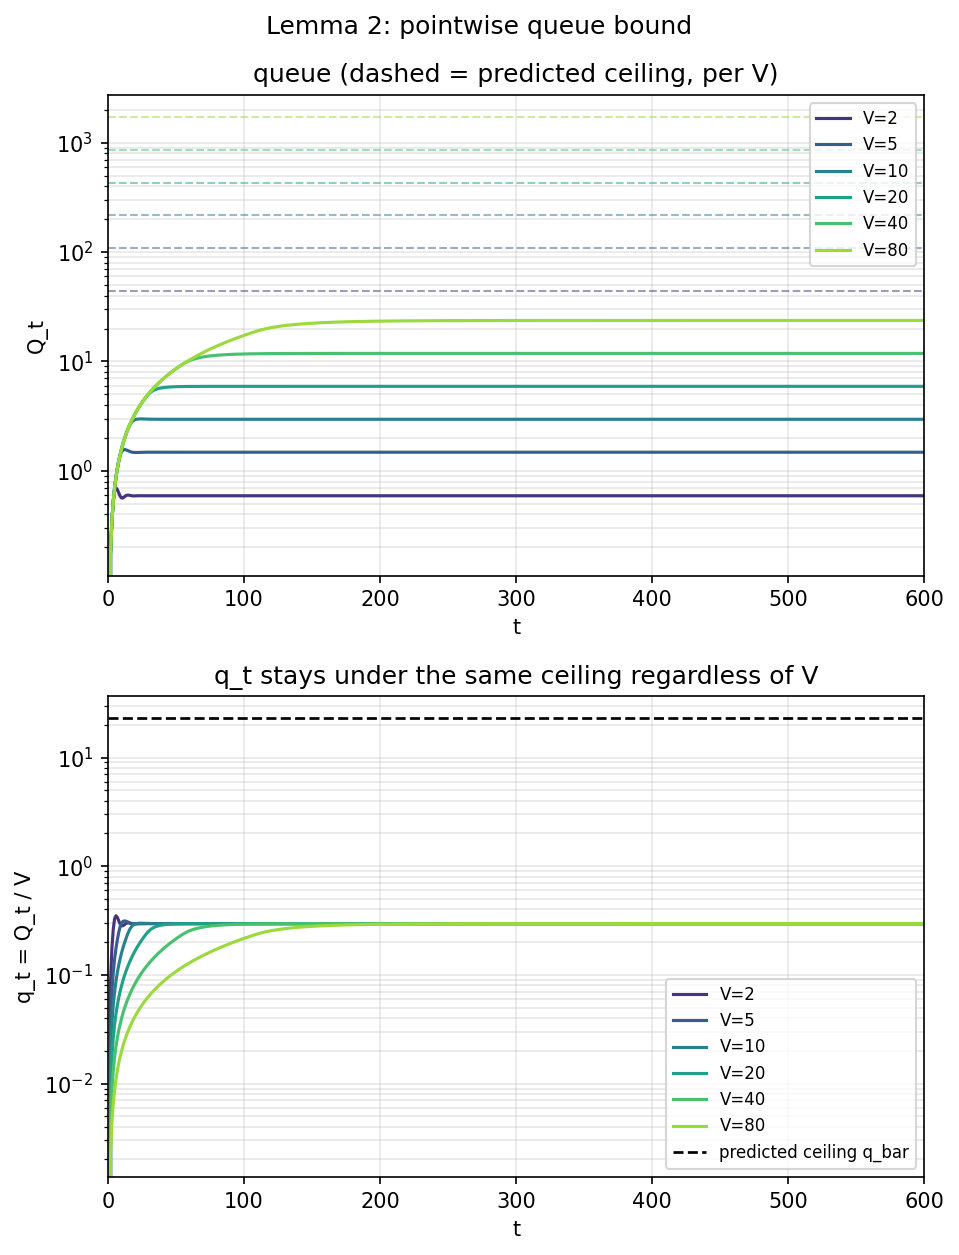
\includegraphics[width=\linewidth,height=195pt,keepaspectratio]{../figures/static/lemma2_queue.png}
    \end{column}
  \end{columns}
\end{frame}

% ------------------------------------------------------------------
\begin{frame}{Theorem 1(a): Time-Average Feasibility}
  \begin{columns}[T]
    \begin{column}{0.48\textwidth}
      \footnotesize
      \[
        \frac{1}{t}\sum_{\tau \le t} h(x_\tau) \;\le\; \frac{\bar Q}{t}
      \]

      \vspace{0.5em}
      \normalsize
      The running average rises, peaks, then decays toward 0 as $t \to T$. Its value at $t=T$ grows with $V$, matching the bound's $V/t$ shape.
    \end{column}
    \begin{column}{0.52\textwidth}
      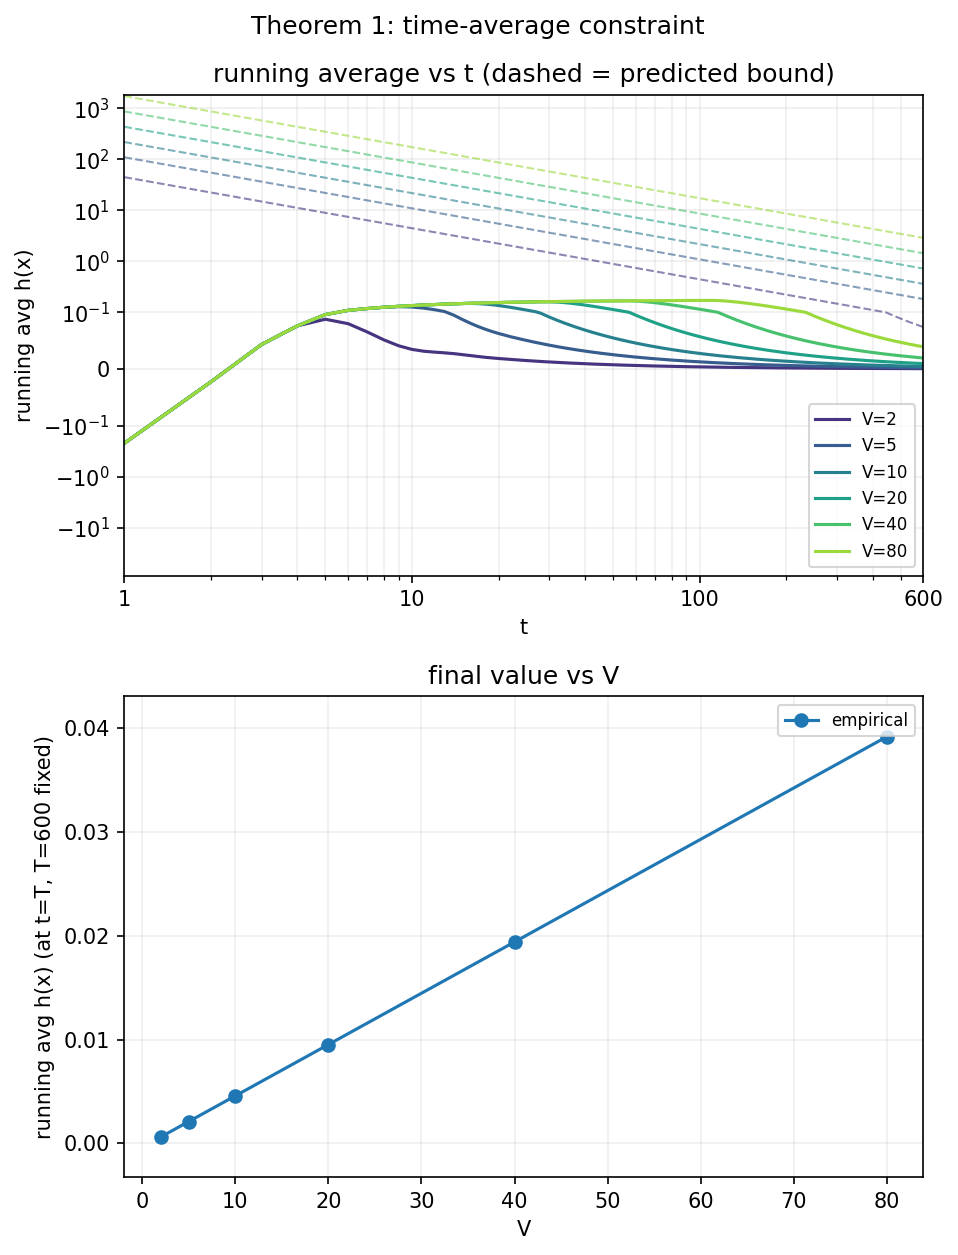
\includegraphics[width=\linewidth,height=195pt,keepaspectratio]{../figures/static/theorem1a_time_average_h.png}
    \end{column}
  \end{columns}
\end{frame}

% ------------------------------------------------------------------
\begin{frame}{Theorem 1(b): Movement Bound}
  \begin{columns}[T]
    \begin{column}{0.48\textwidth}
      \footnotesize
      \[
        \frac{1}{t}\sum_{\tau \le t} \|x_{\tau+1}-x_\tau\|^2 \;\le\; \frac{C_S}{c_0\,t} + \frac{H^2}{c_0\,V}
      \]
      \begin{align*}
        c_0 &= \frac{1}{\eta} - \frac{\rho_f}{2} \\
        \bar q &= \frac{2C_\circ}{\bar\xi} + H \\
        C_S &= P_{\max}(\beta) - P_{\min} + 2\bar q H
      \end{align*}

      \vspace{0.5em}
      \normalsize
      Tracks the predicted shape but sits far inside it -- the bound is conservative, not tight. Final value flattens near a floor as $V$ grows.
    \end{column}
    \begin{column}{0.52\textwidth}
      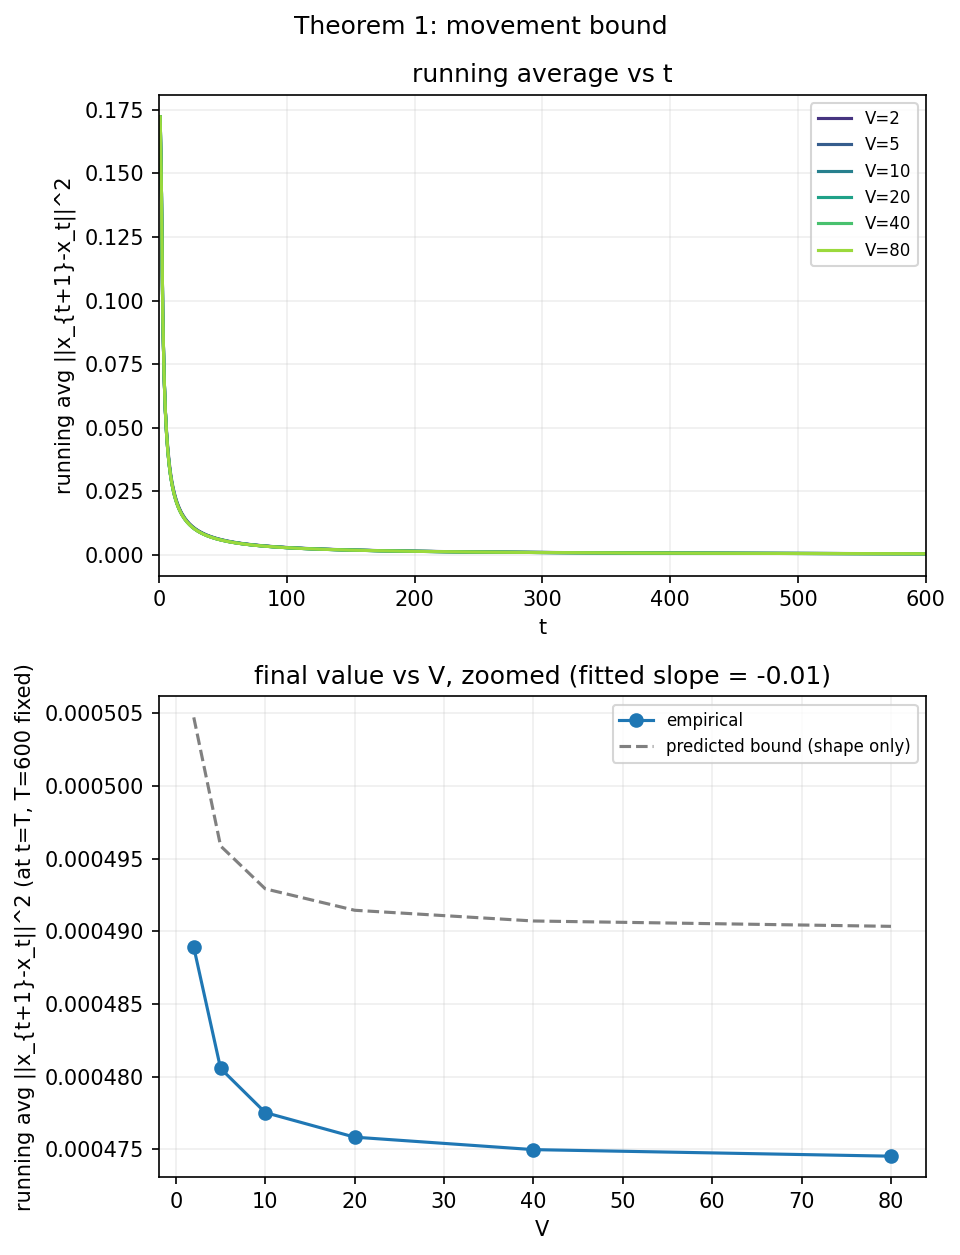
\includegraphics[width=\linewidth,height=195pt,keepaspectratio]{../figures/static/theorem1b_movement.png}
    \end{column}
  \end{columns}
\end{frame}

% ------------------------------------------------------------------
\begin{frame}{Theorem 2: Near-Stationarity}
  \begin{columns}[T]
    \begin{column}{0.48\textwidth}
      \footnotesize
      \[
        \mathbb{E}\big[R(x_{\tau+1},q_\tau)^2\big] \;\le\; A^2\left(\frac{C_S}{c_0\,t} + \frac{H^2}{c_0\,V}\right)
      \]
      \[
        A = \frac{1}{\eta} + 2\gamma \bar q
      \]

      \vspace{0.5em}
      \normalsize
      Inherits Theorem 1(b)'s shape exactly, since $R = A_t \cdot \text{movement}$.
    \end{column}
    \begin{column}{0.52\textwidth}
      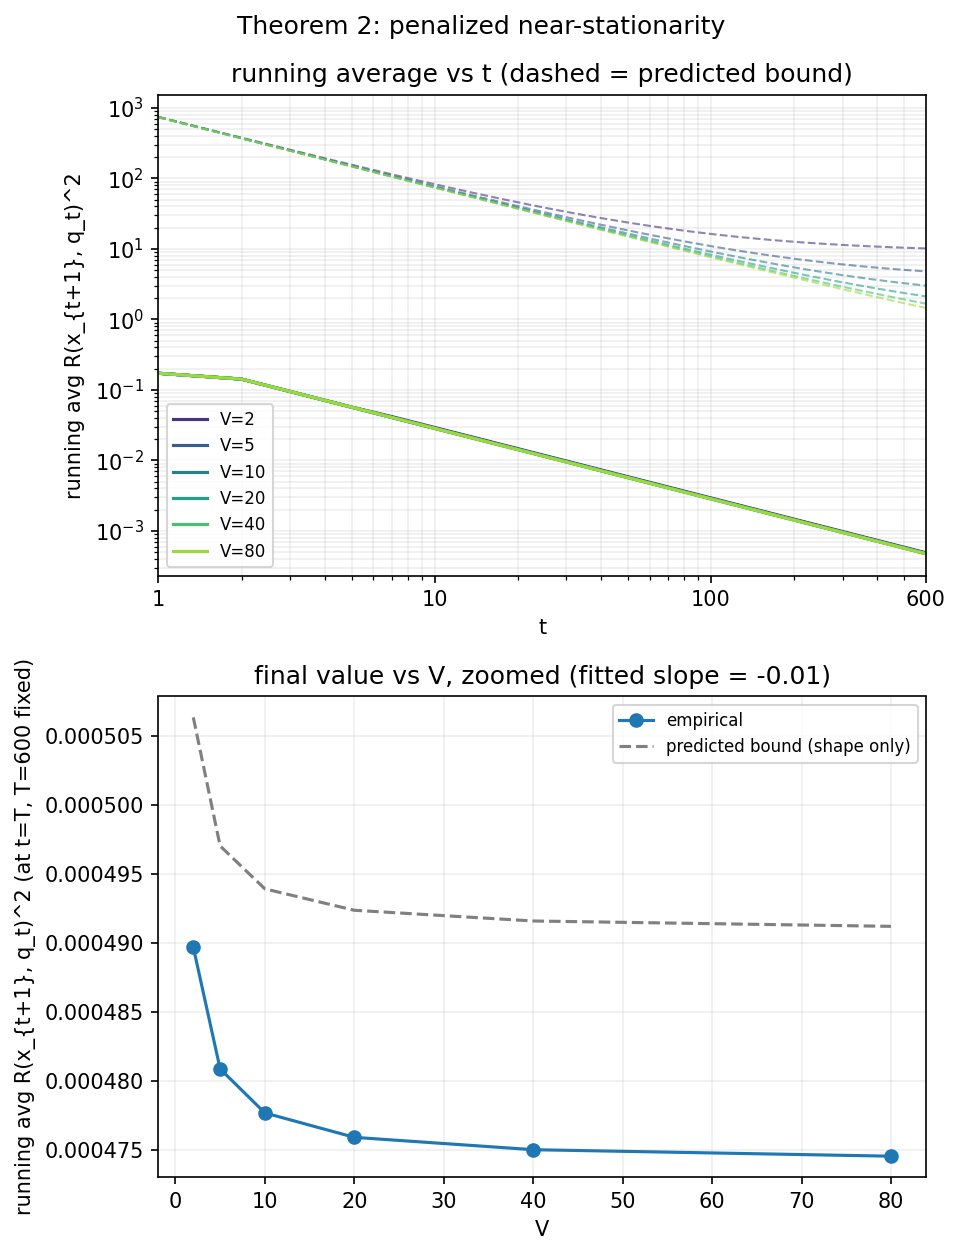
\includegraphics[width=\linewidth,height=195pt,keepaspectratio]{../figures/static/theorem2_residual.png}
    \end{column}
  \end{columns}
\end{frame}

% ------------------------------------------------------------------
\begin{frame}{Theorem 3: Instantaneous Feasibility}
  \begin{columns}[T]
    \begin{column}{0.48\textwidth}
      \footnotesize
      \[
        \mathbb{E}\big[g(x_{\tau+1})\big]_+ \;\le\; \frac{G_g}{\delta_g^{\,2}}\, \mathbb{E}\big[R^2\big], \qquad \delta_g > 0
      \]
      \begin{align*}
        G_g &= R_X^2 - r_g^2 \\
        \kappa_g &= 2\beta r_g \\
        \delta_g &= \kappa_g - L_f - \bar q L_h
      \end{align*}

      \vspace{0.5em}
      \normalsize
      With $\delta_g = 19.47 > 0$ at the default point, the running average of $[g(x)]_+$ sits at floating-point noise ($\sim 10^{-17}$) -- orders below the predicted bound.
    \end{column}
    \begin{column}{0.52\textwidth}
      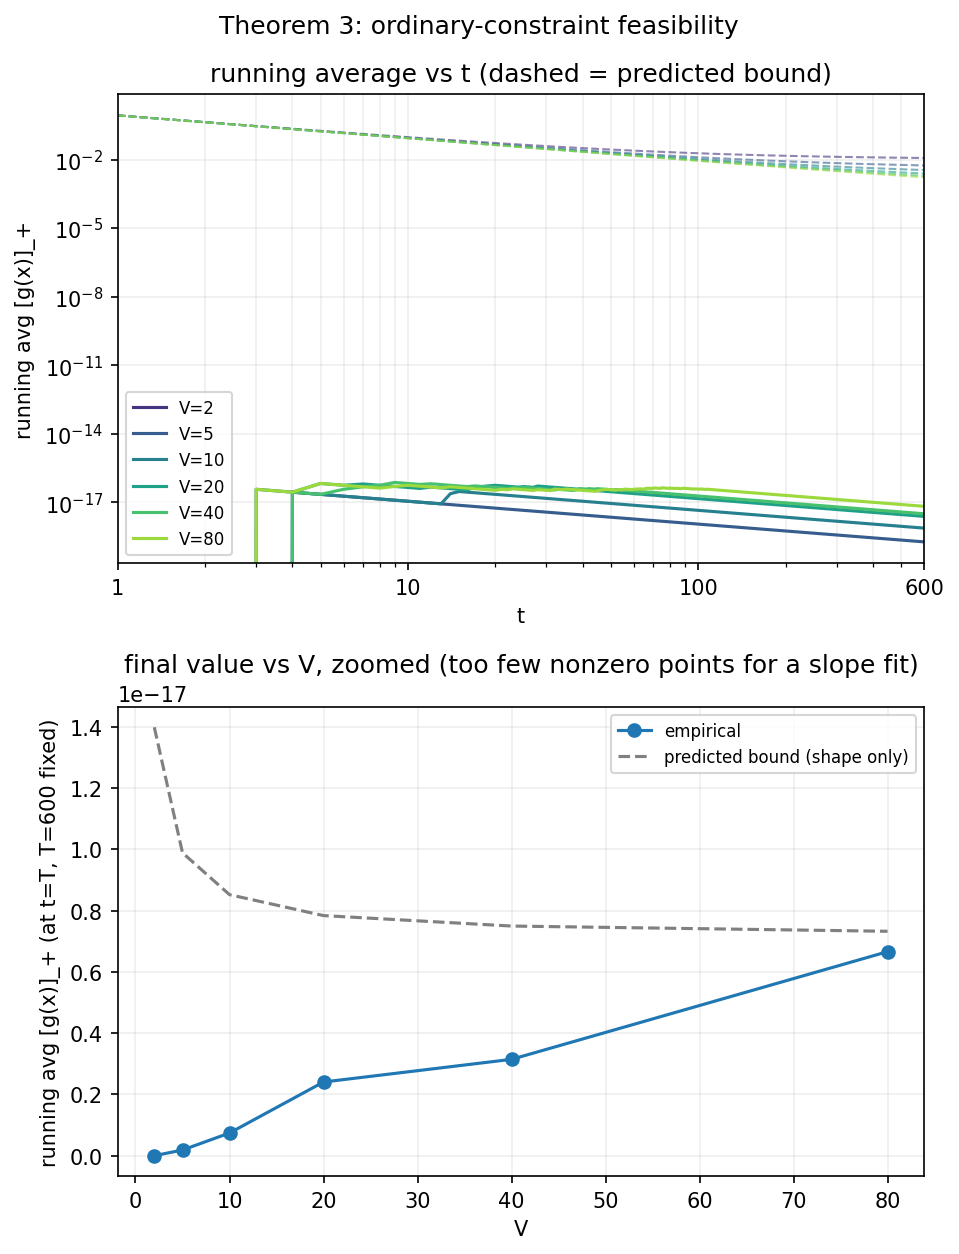
\includegraphics[width=\linewidth,height=195pt,keepaspectratio]{../figures/static/theorem3_violation.png}
    \end{column}
  \end{columns}
\end{frame}

% ------------------------------------------------------------------
\begin{frame}{Corollary 1: Joint Convergence Rate}
  \begin{columns}[T]
    \begin{column}{0.48\textwidth}
      \footnotesize
      At $V = \lceil \varepsilon^{-2} \rceil$, $T = \lceil \varepsilon^{-3} \rceil$:
      \begin{align*}
        \mathbb{E}[R] &= O(\varepsilon) \\
        \mathbb{E}[g]_+ &= O(\varepsilon^2) \\
        |\overline{h}| &= O(\varepsilon)
      \end{align*}

      \vspace{0.5em}
      \normalsize
      Fitted empirical slopes: $R \sim \varepsilon^{2.99}$ and $[g]_+$ at floating-point noise -- both far beating their guarantees. $|\overline{h}| \sim \varepsilon^{0.99}$ matches its $O(\varepsilon)$ guarantee almost exactly.
    \end{column}
    \begin{column}{0.52\textwidth}
      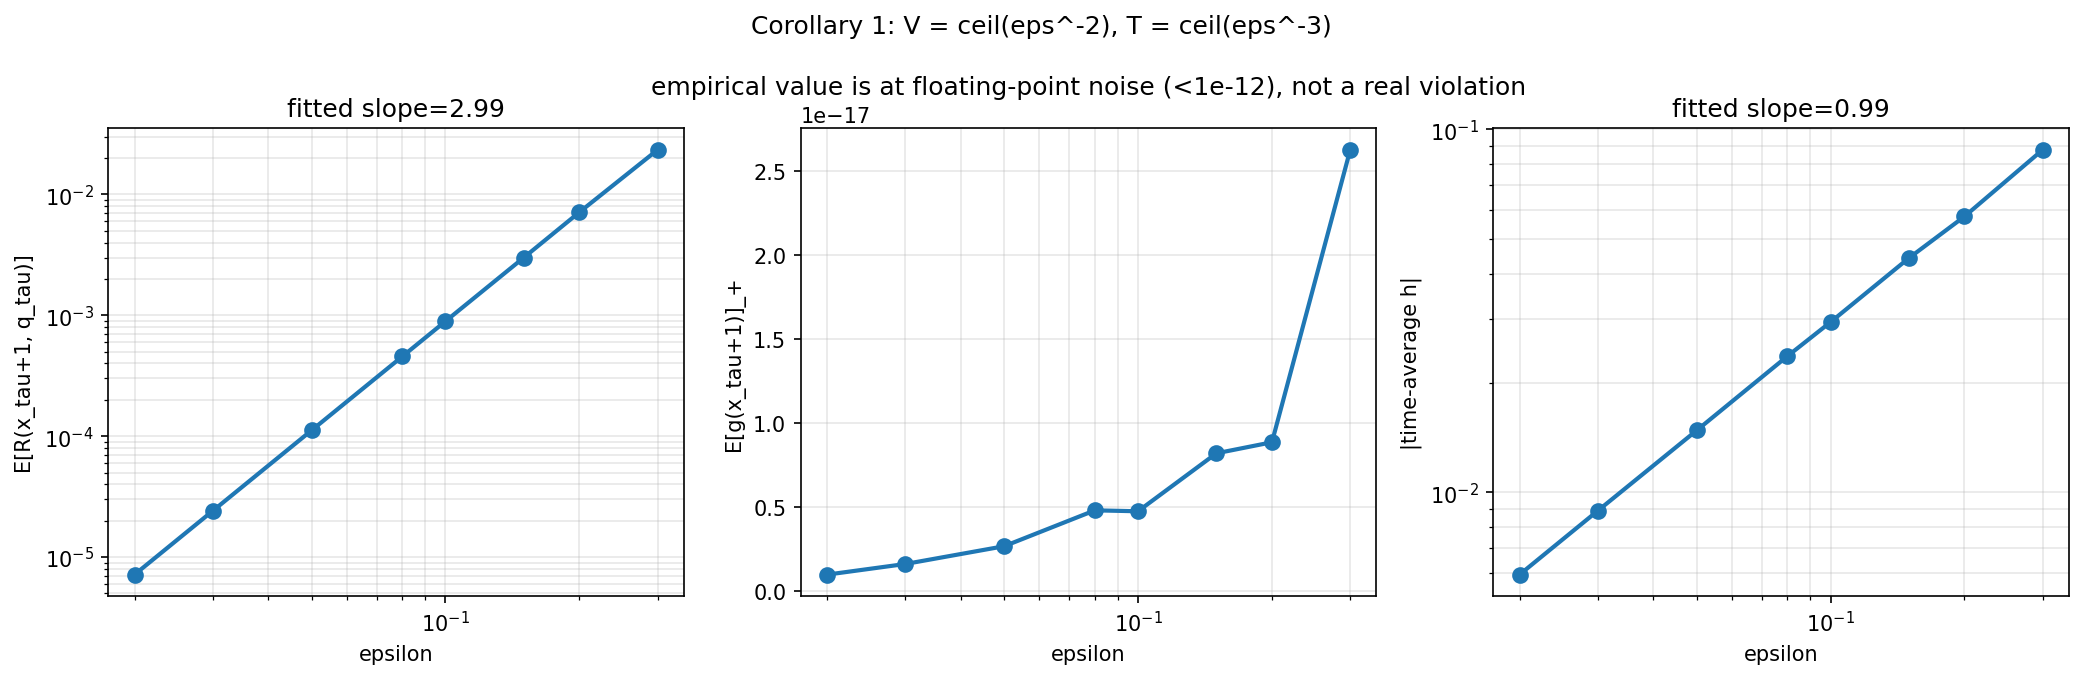
\includegraphics[width=\linewidth]{../figures/static/corollary1_joint_rate.png}
    \end{column}
  \end{columns}
\end{frame}

% ------------------------------------------------------------------
\begin{frame}{A Sample Trajectory}
  \footnotesize
  One run at the default operating point ($\beta=45$, $\gamma=0.04$, $\eta=1.0$, $V=20$, $T=600$), checkpointed every 20 steps.

  \vspace{0.3em}
  \footnotesize
  \centering
  \begin{tabular}{r|rrrrrrr}
    $t$ & $Q_t$ & $q_t$ & $f(x_t)$ & $P(x_t)$ & avg $h$ & avg mv$^2$ & avg $g_+$ \\
    \hline
    40  & 5.7513 & 0.2876 & -0.2620 & -0.2620 & 0.1383 & 7.14e-03 & 3.61e-17 \\
    80  & 5.9270 & 0.2964 & -0.2537 & -0.2537 & 0.0713 & 3.57e-03 & 1.80e-17 \\
    120 & 5.9278 & 0.2964 & -0.2536 & -0.2536 & 0.0476 & 2.38e-03 & 1.20e-17 \\
    160 & 5.9278 & 0.2964 & -0.2536 & -0.2536 & 0.0357 & 1.78e-03 & 9.02e-18 \\
    200 & 5.9278 & 0.2964 & -0.2536 & -0.2536 & 0.0285 & 1.43e-03 & 7.22e-18 \\
    240 & 5.9278 & 0.2964 & -0.2536 & -0.2536 & 0.0238 & 1.19e-03 & 6.01e-18 \\
    280 & 5.9278 & 0.2964 & -0.2536 & -0.2536 & 0.0204 & 1.02e-03 & 5.15e-18 \\
    320 & 5.9278 & 0.2964 & -0.2536 & -0.2536 & 0.0178 & 8.92e-04 & 4.51e-18 \\
    360 & 5.9278 & 0.2964 & -0.2536 & -0.2536 & 0.0159 & 7.93e-04 & 4.01e-18 \\
    400 & 5.9278 & 0.2964 & -0.2536 & -0.2536 & 0.0143 & 7.14e-04 & 3.61e-18 \\
    440 & 5.9278 & 0.2964 & -0.2536 & -0.2536 & 0.0130 & 6.49e-04 & 3.28e-18 \\
    480 & 5.9278 & 0.2964 & -0.2536 & -0.2536 & 0.0119 & 5.95e-04 & 3.01e-18 \\
    520 & 5.9278 & 0.2964 & -0.2536 & -0.2536 & 0.0110 & 5.49e-04 & 2.78e-18 \\
    560 & 5.9278 & 0.2964 & -0.2536 & -0.2536 & 0.0102 & 5.10e-04 & 2.58e-18 \\
    600 & 5.9278 & 0.2964 & -0.2536 & -0.2536 & 0.0095 & 4.76e-04 & 2.41e-18 \\
  \end{tabular}

  \vspace{0.3em}
  \footnotesize
  \raggedright
  $Q_t$ saturates by $t\approx100$; $f(x_t)=P(x_t)$ at every single step (the penalty is never active, not just on average); avg $h$ and avg movement$^2$ keep decaying toward 0.
\end{frame}

% ------------------------------------------------------------------
\begin{frame}{One Run: f, h, Q, P vs t}
  \centering
  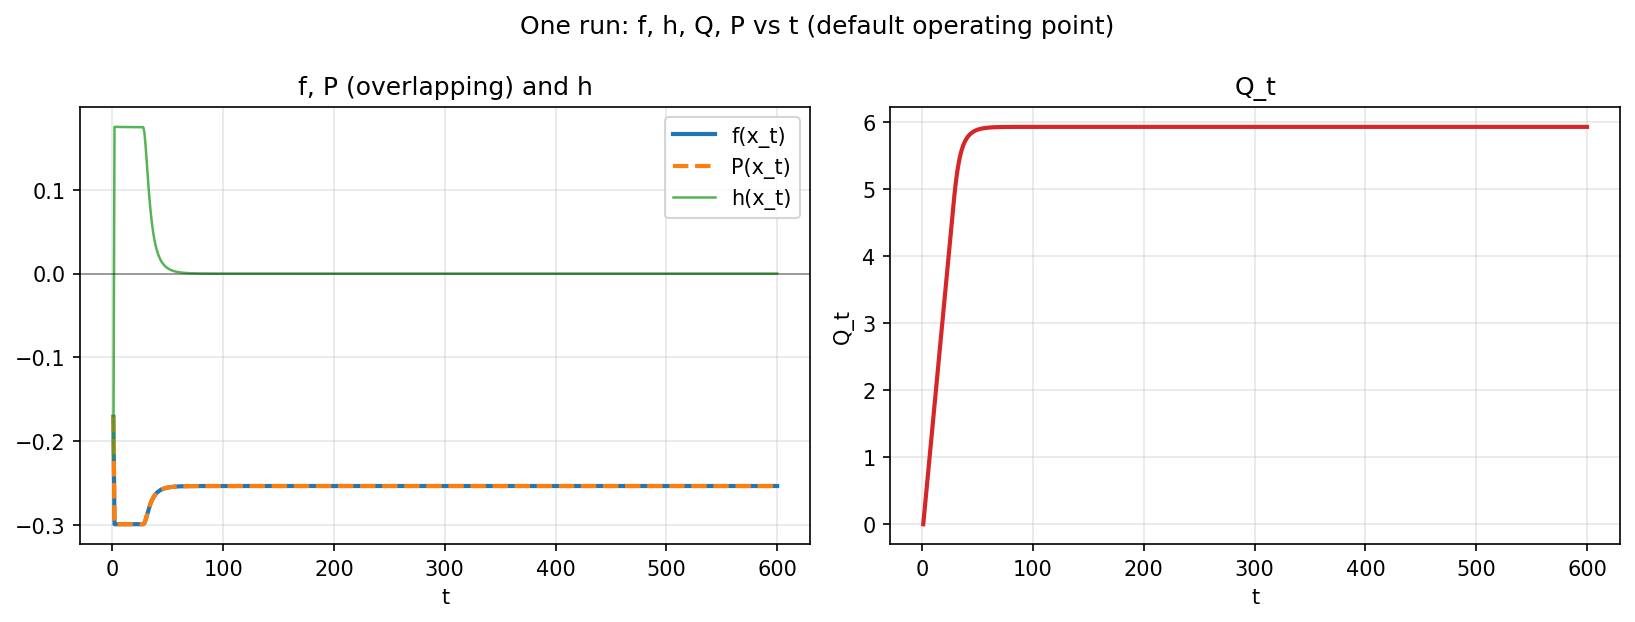
\includegraphics[width=0.95\textwidth]{../figures/static/trajectory_overview.png}

  \vspace{0.3em}
  \footnotesize
  \raggedright
  $f(x_t)$ and $P(x_t)$ overlap exactly for the whole run -- $g(x_t)$ never actually crosses 0 at any single step, so $\beta[g(x_t)]_+ = 0$ throughout, not just in the running average. $h(x_t)$ spikes positive early (while $Q_t$ is still small and the algorithm hasn't yet been penalized for it), then settles near 0 once $Q_t$ saturates.
\end{frame}

% ------------------------------------------------------------------
\begin{frame}{The Price of Feasibility}
  \centering
  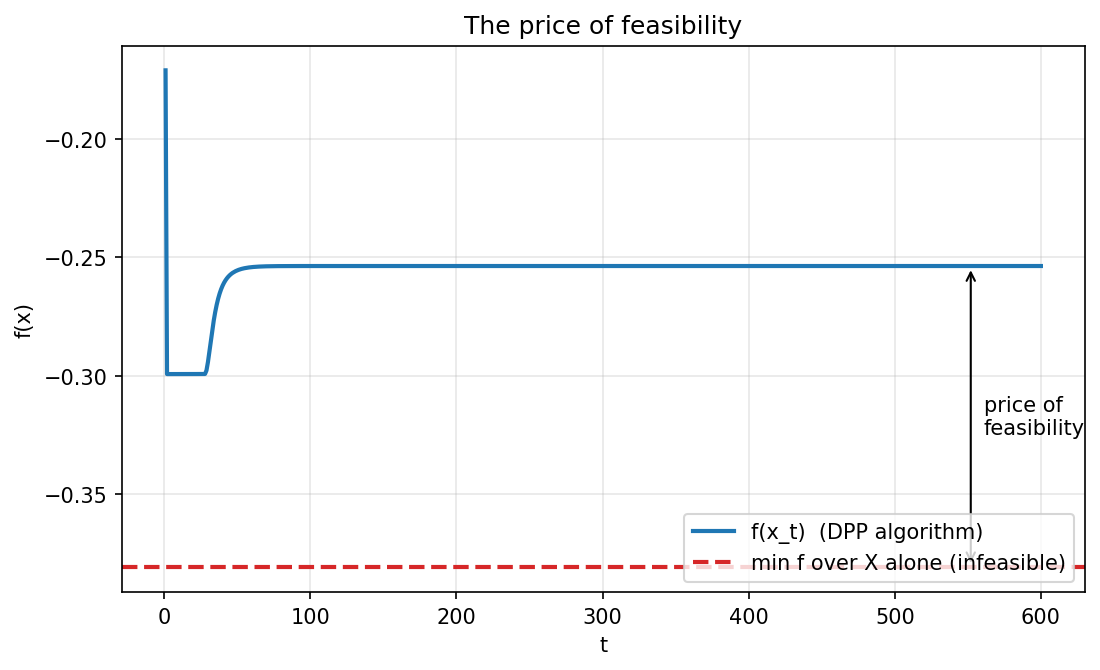
\includegraphics[width=0.75\textwidth]{../figures/static/price_of_feasibility.png}

  \vspace{0.3em}
  \footnotesize
  \raggedright
  Minimizing $f$ alone over $X$ (ignoring $h$, $g$ entirely) reaches $f=-0.3808$ -- but at $g=+0.4375$, $h=+0.6159$: badly infeasible. The DPP algorithm settles at $f=-0.2536$ instead, about $0.127$ worse, in exchange for $h(x_t)\approx0$ and $g(x_t)\le0$ throughout. $Q_t$ is exactly the mechanism paying that price -- it pulls $x$ away from $f$'s true minimum toward the feasible region.
\end{frame}

\end{document}
